\documentclass[fullpage]{article}

%\setlength {\topmargin} {-1in}

%\setlength {\textheight} {8.6in}

%\setlength{\parindent}{1cm}

\usepackage{amsmath, amsfonts}
\usepackage[margin=1in]{geometry}
\usepackage{amssymb}
\usepackage{amsthm}
\usepackage{amsmath}
\usepackage{multirow}
\usepackage{verbatim}
\usepackage{listings}
\usepackage{color}
\usepackage{hyperref}
\usepackage{blindtext}
\usepackage{cancel}
\usepackage{float}
\usepackage{enumitem}
\usepackage{graphicx}    %  in the preamble
%\usepackage[acronym]{glossaries}

\usepackage[table]{xcolor}
\setlength{\tabcolsep}{18pt}
\renewcommand{\arraystretch}{1.5}
\renewcommand{\labelenumi}{\theenumi.}
\renewcommand{\labelenumii}{\theenumii.}
\renewcommand{\labelenumiii}{\theenumiii.}
\newcommand{\be}{\begin{enumerate}}
\newcommand{\ee}{\end{enumerate}}
\newcommand{\bi}{\begin{itemize}}
\newcommand{\ei}{\end{itemize}}
\newcommand{\bc}{\begin{center}}
\newcommand{\ec}{\end{center}}
\newcommand{\bv}{\begin{verbatim}}
\newcommand{\ev}{\end{verbatim}}
\newcommand{\ba}{\begin{align*}}
\newcommand{\ea}{\end{align*}}
\newcommand{\beq}{\begin{equation*}}
\newcommand{\eeq}{\end{equation*}}
\newcommand{\bs}{\begin{split}}
\newcommand{\es}{\end{split}}
\newcommand{\mname}[1]{\mbox{\sf #1}}
\newcommand{\pnote}[1]{{\langle \text{#1} \rangle}}
\renewcommand{\labelenumii}{\theenumii.}

\begin{comment}
\makeglossaries
\newacronym{SRS}{System Requirements Specification}
\newacronym{UPC}{Universal Product Code}
\newacronym{ISBN}{International Standard Book Number}
\newacronym{GUI}{Graphical User Interface}
\newacronym{NFR}{Non-Functional Requirements}
\end{comment}
\begin{document}

\vspace*{\fill}
\begin{center}

  {\Huge \textbf{System Requirements}}\\
\hrulefill\\[2mm]
  {\huge \textbf{Book Bazar}}\\[2mm]
{\large \today}\\[15mm]
{\large
\underline{\textbf{Group 6}}\\
\begin{tabular}{ c c }

 Caleb Mech & mechc2\\ 
 David Thompson & thompd10\\
 Matthew Williams & willim36\\
 Ahmed Al Koasmh & alkoasma\\
 Harsh Mahajan	& mahajanh    
\end{tabular}
}

\end{center}

\vspace*{\fill}

%-----------END OF TITLE PAGE-------------------------------------------------------------
\newpage
\begingroup
\hypersetup{hidelinks}
\tableofcontents

\listoffigures
\listoftables
\endgroup
\newpage

\section{Table of Revisions}
\begin{table}[h]
\centering
\begin{tabular}{| l | c | p{4cm}| p{5cm}|}
\hline
 \rowcolor{lightgray} 
\textbf{Version} & \textbf{Date(dd.mm.yyy)} &\textbf{Author(s)} &\textbf{Description}\\
\hline
0 & 11.10.2021 & Caleb Mech\newline Ahmed Al Koasmh\newline  David Thompson \newline Matthew Williams \newline Harsh Mahajan & First version compiled.\\
\hline
1 & 15.10.2021 & Ahmed Al Koasmh\newline David Thompson \newline Harsh Mahajan & Existing version editing with feedback from David and Ahmed. \newline Major edits: Addition of NFRs; Revision of Use-Case Diagram.\\
\hline
2 & 16.10.2021 & Caleb Mech \newline David Thompson \newline Mathew Williams \newline Ahmed Al Koasmh & Behavior Overview \& Requirements Likelihood to Change added. Context diagram edited.\\
\hline
3&17.10.2021& Harsh Mahajan &Document edited for corrections \& References added.\\
\hline
4 & 18.10.2021& David Thompson \newline Ahmed Al Koasmh & Edited Fuctional Requirements to match conventions; added ``shall.''\\
\hline
5 & 19.10.2021 & Harsh Mahajan & Edited Use-Case Diagram to match TA's feedback.\\
\hline
6 & 25.02.2022 & Caleb Mech & Edited user and authentication requirements to match system design.\\
\hline
\end{tabular}
\caption{Table of Revisions}

\end{table}

\section{Purpose}
The motivation for this project is to create an application that allows McMaster students to conveniently buy and sell textbooks in a secure marketplace. Currently, students use online websites like Facebook (https://www.facebook.com/groups/macusedtexts) or the campus store’s buyback program \\ (https://campusstore.mcmaster.ca/information/guaranteed-buyback.html, suspended because of COVID) to sell their books. These current solutions are either disorganized or take a cut of the transaction. Book Bazar aims to create an organized marketplace that allows users to sell books for a better price than at the campus store.

The purpose of this System Requirements Specification (SRS) is to provide a clear overview of the project’s functional and non-functional requirements that are relevant to the application’s stakeholders.\\ % Comment about not needing non-functional requirements removed since TA said we need them
\newline
\small{ \textbf{NOTE:} Book Bazar's website where all the books to be sold are listed, is referred to as \textit{marketplace} in certain parts of this document.}
\newpage
\section{Scope}
The scope for the project covers the following application features:
\be
	\item An authentication and authorization platform that verifies McMaster students and allows them to log into and use the application.
	\item A marketplace system that uses information from the campus store and allows users to:
		\bi
			\item Post about and categorize books that they would like to sell.
			\item Search for books that they would like to purchase.
		\ei
	\item A system that allows buyers and sellers to privately contact each other, agree on a price, and choose where they would like to meet.
	\item The application will be accessible from any device with a modern browser (phone, tablet, desktop, etc.) to provide the best experience.
\ee

%Not including the scalable part as we're movig it to a stretch goal.

\section{Context Diagram}
\label{sec:context}
% Ahmed: Can we change "University Library" to "Campus Bookstore"
% Ahmed: Is the arrow "Book Listings" from "Seller" to "Book System" the same content as "Book Listings" from "University Library" to "Book System". If they are not the same, I would recommend we change "Book Listings" for Seller and Buyers arrows to "Book Postings".
%SHOULD WE SHOW BOUNDARIES?

\begin{figure}[h!]
    \centering
     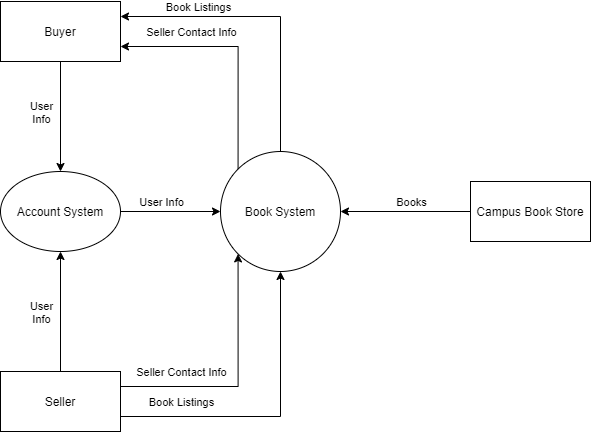
\includegraphics[width=0.75\textwidth]{a.png}
    \caption{Book Bazar Context Diagram}
    \label{ContextDiagram}
\end{figure}

\section{Constants, Monitored and Controlled Variables}
%SHOULD WE REMOVE THIS?
% David: no we do need this per the discussion with Dr Wassyng. I think the only other thing that we might need to mention is that the OS and the browser handle keypresses and mouse interaction? I guess we also need to convert the price the seller inputs from a string into an IEEE-754 double precision floating point number
The Book Bazar application will not be using any elements from the physical world, like temperature, length, speed, etc., which require high precision when manipulating within the software. Elements from the physical world that Book Bazar will be using will be the Universal Product Code (UPC) code of books, information of users and the prices of books. All of these elements will be treated as constants and will not undergo changes.

%Help refining / sounding a bit more technical?
\newpage

\section{Behaviour Overview}
\begin{comment}
This specification document specifies a software system that allows McMaster University students to buy and sell used textbooks. Students who have used textbooks that they want to sell can create a posting/listing on the system by entering the UPC/ISBN13 code of the book and adding their desired sell price. Students who are looking to buy books can view the listings that the sellers created. The buyers will be able to filter postings/listings in order to quickly find what they are looking for. When a buyer finds a posting for a textbook that they want, they will be able to send a message to the seller in order to confirm the price and schedule a time to meet up to sell/buy the textbook. A book seller will be able to remove their posting if they decide not to sell the textbook or manage to find a buyer some other way.
\end{comment}
\noindent This specification document specifies a software system that allows McMaster University students to buy and sell used textbooks. Here is an overview of the system's behaviour in reference to the \hyperref[sec:context]{context diagram in section 4}:

\begin{table}[H]
\flushleft
\begin{tabular}{|p{4cm}|p{10cm}|}
\hline
 \rowcolor{lightgray} 
\textbf{Boundaries} & \textbf{Behaviour Description}\\
\hline
$\textit{Campus Book Store} \rightarrow \textit{Book System}$ & The book system retrieves relevant book information from the campus book store which allows the system to sort book data based on relevant categories.\\
\hline
$\textit{Seller} \rightarrow \textit{Book System}$ & Students who have used textbooks that they want to sell can create a posting/listing on the system by entering the UPC/ISBN13 code of the book and adding their desired sell price. A book seller will be able to remove their posting from the system if they decide not to sell the textbook or manage to find a buyer some other way.\\
\hline
$ \textit{Seller} \rightarrow \textit{Account System}$ \newline $Buyer \rightarrow \textit{Account System}$ \newline $\textit{Account S.} \rightarrow \textit{Book S.}$ &Buyers and sellers can store their confidential information including authentication and authorisation parameters within the Account System. Relevant information will be shared with the book system accordingly.\\
\hline
$\textit{Book System} \rightarrow \textit{Buyer}$ & Students who are looking to buy books can view the listings that the sellers created and retrieve them from the book system. The buyers will be able to filter postings/listings in order to quickly find what they are looking for. When a buyer finds a posting for a textbook that they want, they will have can retrieve the seller's contact information, and they will be able to send a message to the seller in order to confirm the price and schedule a time to meet up to sell/buy the textbook.\\
\hline
\end{tabular}
\caption{Boundary Descriptions and System Behaviour}
\end{table}


\newpage

\section{Use-Case Diagram}
\begin{figure}[h]
    \centering
    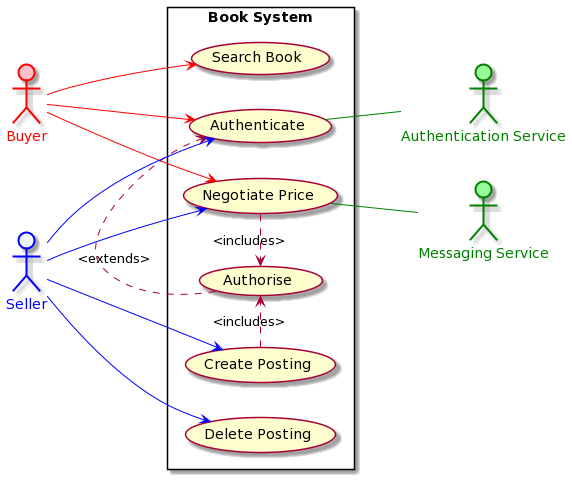
\includegraphics[width=1.05\textwidth]{b.png}
    \caption{Book Bazar User Diagram}
    \label{UserDiagram}
\end{figure}

\section{Normal/Undesired Operations}

\begin{table}[H]
\flushleft
\begin{tabular}{|c|p{3cm}|p{4cm}|p{4cm}|}
\hline
 \rowcolor{lightgray} 
\textbf{Event} & \textbf{Operation Type} &\textbf{Description} &\textbf{Course of Action}\\
\hline
\multirow{4}{*}{Sign-in} & Normal Operation & User’s university email address is validated. & -\\
& Undesired Event & The submitted email is invalid. & The user will be informed that their email is invalid and will be prompted to sign in again.\\
& Undesired Event & The user attempts to log in with an incorrect password more than 5 times. & Redirect the user to set up a new password before logging into the application.\\
& Undesired Event & The user visits a forbidden page on the website without being authenticated. & Redirect the user to a login page.\\
\hline
\multirow{3}{*}{Book Listing}& Normal Operation &The user submits a book, and it is listed on the website.&-\\
& Undesired Event &The submitted book is not valid.&The listing will not be completed, and the user will be prompted to try listing again.\\
& Undesired Event &The service which provides information on a book given the International Standard Book Number (ISBN) does not recognize the ISBN.& The user will be prompted to manually enter the details of the book, such as the title, edition, and authors.\\
& Undesired Event &A book posting remains on the application for 20 days without a sale occurring. & On the 15th day, provide a warning notification to the user asking them if they would still like the posting to be placed. If no response is received by the 20th day, the application archives the posting and removes it from the marketplace.\\
\hline
\end{tabular}
\caption{Types of Operations, Part 1}
\end{table}
\begin{table}[H]
\flushleft
\begin{tabular}{|c|p{3cm}|p{4cm}|p{4cm}|}
\hline
 \rowcolor{lightgray} 
\textbf{Event} & \textbf{Operation Type} &\textbf{Description} &\textbf{Course of Action}\\
\hline
\multirow{3}{*}{Site Navigation}& Normal Operation &Users will use the Graphical User Interface (GUI) to navigate the site from any supported browser.&-\\
& Undesired Event &The user visits the application from an unsupported browser.& Display an error message listing browsers that are supported.\\
& Undesired Event &The user visits a non-existent page.&Display an error message listing that the page was not found.\\
\hline
\end{tabular}
\caption{Types of Operations, Part 2}
\end{table}

\section{Functional Requirements}

\subsection{Posting Book}
\begin{table}[h!]
\flushleft
\begin{tabular}{|c|p{6cm}|p{6cm}|}
\hline
 \rowcolor{lightgray}
\textbf{Requirement} & \textbf{Description} & \textbf{Rationale} \\
\hline
FR1 &The system shall allow sellers to post books by manually inputting book information.& -\\
\hline
FR2&The system shall allow sellers to post books by scanning a -UPC barcode and filling out the remaining information. & This will allow users to easily post books without manually filling out its details.\\
\hline
FR3 & System shall allow sellers to delete their posting.& The seller may no longer be interested in selling the book.\\
\hline
FR4 &  The system shall allow sellers to view the price the book is currently being sold for at the Campus Store. & Sellers may be interested in selling their book for a percentage of the price they originally paid while taking the Campus Store price into account.\\
\hline
FR19 & System shall allow sellers to edit their posting.& The seller may want to change the price or edit their posting.\\
\hline
\hline
\end{tabular}
\caption{Requirements for Posting Book}
\end{table}
\newpage
\subsection{Buying Book}
\begin{table}[h!]
\flushleft
\begin{tabular}{|c|p{6cm}|p{6cm}|}
\hline
 \rowcolor{lightgray} 
\textbf{Requirement} & \textbf{Description} & \textbf{Rationale} \\
\hline
FR5 &The system shall allow buyers to find books for a specified course code. & Buyers may want to find the books available for a courses that they are taking.\\
\hline
FR6&The system shall allow buyers to find books by book name. & Buyers may be looking for a specific book.\\
\hline
FR7 &The system shall allow buyers to initiate a chat with sellers using Microsoft Teams.
% or another 3rd party chat service
& This way, the users can continue enjoying the secure nature of the platform. \\
% Ahmed: This may need to be changed to "the users can choose the most convenient way for them to contact each other."
\hline
FR8 & The system shall allow buyers to contact sellers using email. & Not all buyers may be comfortable with a chat-feature and may prefer something more formal.\\
\hline
FR9 & The system shall only give sellers' information to authorized buyers. & Sellers may be uncomfortable with their name, photo, and contact information being available on the open internet. Only allowing authorized buyers will reduce privacy and spam concerns.\\
\hline
FR10 & The system shall allow buyers to find books at the campus store. &The selection of used books may not satisfy the buyer. In this case, they can opt to purchase the book from the campus store.\\
\hline
\end{tabular}
\caption{Requirements for Buying Book}
\end{table}

\newpage
\subsection{Authentication System}
\begin{table}[h!]
\flushleft
\begin{tabular}{|c|p{6cm}|p{6cm}|}
\hline
 \rowcolor{lightgray} 
\textbf{Requirement} & \textbf{Description} & \textbf{Rationale} \\
\hline
FR11 &The system shall allow new users to create an account.& Users will need an account in order to use the website as verified users.\\
\hline
FR12&The system shall allow users to delete their account. & Users may wish to no longer have their information on the website.\\
\hline
FR13 & The system shall provide tips regarding safe interaction between buyers and sellers. & -\\
\hline
FR15 &The system shall allow existing users to login.& -\\
\hline
FR16 &The system shall allow authenticated users to logout.& -\\
\hline
FR17 &The system shall allow authenticated users to update their user information.& Users may wish to modify their account information such as name or profile image\\
\hline
FR18 &The system shall prevent users modifying user information that is not their own.& -\\
\hline
\end{tabular}
\caption{Requirements for the Authentication System}
\end{table}

\section{Functional Requirements Likelihood of Change}

\textbf{NOTE:} All unlisted requirements are very unlikely to change as they are imperative to our project goals.
\begin{table}[h!]
\flushleft
\begin{tabular}{|c|c|p{6cm}|}
\hline
 \rowcolor{lightgray} 
\textbf{Requirement} & \textbf{Likelihood (1-5)} & \textbf{Rationale} \\
\hline
FR7 & 3 & We may have difficultly interfacing with Microsoft Teams as a chat platform for connecting users. \\
\hline
\end{tabular}
\caption{Functional requirements likely to change}
\end{table}


\section{Non-Functional Requirements (NFR)}


\subsection{Look and Feel Requirements}
\begin{table}[h!]
\flushleft
\begin{tabular}{|c|p{6cm}|p{6cm}|}
\hline
 \rowcolor{lightgray} 
\textbf{Requirement} & \textbf{Description} & \textbf{Rationale} \\
\hline
NFR1 &The application GUI must have a self-consistent design language; a GUI component that appears in multiple contexts should have a similar look and feel in all contexts.& This will provide a system that users feel is trustworthy and intuitive.\\
\hline
\end{tabular}
\caption{NFR: Look and Feel}
\end{table}

\newpage

\subsection{Usability Requirements}
\begin{table}[h!]
\flushleft
\begin{tabular}{|c|p{6cm}|p{6cm}|}
\hline
 \rowcolor{lightgray} 
\textbf{Requirement} & \textbf{Description} & \textbf{Rationale} \\
\hline
NFR2 & It should take no more than 10 minutes for a new user to create an account and make a used book listing. & - \\
\hline
NFR3 & It should take no more than 5 minutes for a new user to find a book that they are looking for. & -\\
\hline
\end{tabular}
\caption{NFR: Usability}
\end{table}



\subsection{Performance Requirements}
\begin{table}[h]
\flushleft
\begin{tabular}{|c|p{6cm}|p{6cm}|}
\hline
 \rowcolor{lightgray} 
\textbf{Requirement} & \textbf{Description} & \textbf{Rationale} \\
\hline
NFR4 & The $95^{\text{th}}$ percentile of a sample of page load times must be under 3 seconds & -\\

% David: This might be determined by the client that is loading the website,
% as well as the network speed.
% I think that we should provide a description of the computer and network that should be able to load
% the website within 3 seconds.
% Here is a rough idea of what I have in mind:
% 
\hline
NFR5 &Server must support 1000 concurrent users.& - \\ %is this achievable?
% David: I think that our budget directly determines how many concurrent users we can support.
% I believe we will be able to scale our website and backend (code that connects webpage and database) horizontally,
% which means we can rent more computers in order to increase the amount of users we support.
% Renting more computers costs more money, but could be cheaper then renting a faster computer to support more users.
% The more limiting factor might be our database,
% since from by understanding the only way to speed a relational database up is to run the database on a faster computer.
% Here is the pricing for Amazon RDS: https://aws.amazon.com/rds/postgresql/pricing/?pg=pr&loc=3
\hline

NFR6 & A book must be listed to the website within 3 seconds of submission and visible to other users on the website.&- \\
% David: I think we should add something to the effect of: "and this change should be visible from other
% users on the website" just to be a bit more specific
%Harsh: Added.
\hline
NFR7& The application must have an availability rate of 99.9\% within any allocated time frame.&-\\
% David: Is this achievable? I think we should promise/aim for a little lower, and then hope to overachieve
\hline
% NFR7& If a user is signed up for notifications (email, phone, etc.), the application should push them out within 3 seconds.&-\\
% David: I think that 3 seconds might be a bit too low of a latency to achieve with SMS (texting), so I searched through the Twilio docs for their SLA on latency for text messaging but I didn't find any concrete numbers. I guess we can adjust in the future when we know better what to expect?
\end{tabular}
\caption{NFR: Performance}
\end{table}

\subsection{Operational and Environmental Requirements}
\begin{table}[h!]
\flushleft
\begin{tabular}{|c|p{6cm}|p{6cm}|}
\hline
 \rowcolor{lightgray} 
\textbf{Requirement} & \textbf{Description} & \textbf{Rationale} \\
\hline
NFR8 & The application should be able to be operated by at least one person who has limited system administration experience. & -\\
\hline
NFR9&The operational costs of the application should be minimized. & -\\
\hline
NFR10 &Users can access all functionality with any browser with $>2\%$ market-share in Canada \cite{website} & This way, the website is accessible to the majority of users.\\
\hline
\end{tabular}
\caption{NFR: Operation and Enviroment}
\end{table}


\subsection{Maintainability and Support Requirements}
\begin{table}[h!]
\flushleft
\begin{tabular}{|c|p{6cm}|p{6cm}|}
\hline
 \rowcolor{lightgray} 
\textbf{Requirement} & \textbf{Description} & \textbf{Rationale} \\
\hline
NFR11 & The application should be maintainable by at least one developer who is skilled in the technologies used to develop the application. & -\\
\hline
\end{tabular}
\caption{NFR: Support and Maintainability}
\end{table}


\subsection{Security Requirements}
\begin{table}[h!]
\flushleft
\begin{tabular}{|c|p{6cm}|p{6cm}|}
\hline
 \rowcolor{lightgray} 
\textbf{Requirement} & \textbf{Description} & \textbf{Rationale} \\
\hline
NFR12& Attackers should be unable to access confidential data stored by the application's servers. &- \\% David: Looking back at this, I need to be more clear. Also, this is very similar to the first security requirement
\hline
NFR13& Attackers should be incapable of running arbitrary code on any of the servers running components of the application. &- \\% Ahmed: Instead of computers, can we say "servers"?
% David: Yep: I changed it
\hline
NFR14 & Attackers should be unable of intercepting or monitoring data and events exchanged between the user's device and the application servers, given that neither the application servers nor the user's device are compromised. & - \\% Ahmed: Can we change the wording? If someone has control over your device, there is little we can do on our end (besides timing out the session and protecting the username/password). Instead of "generated by users...", can we say "exchanged by the user's device and the application server".
% David: Yes; I like this wording better, and I'll adapt this to the wording
\hline
\end{tabular}
\caption{NFR: Safety}
\end{table}

\subsection{Cultural Requirements}
\begin{table}[h!]
\flushleft
\begin{tabular}{|c|p{6cm}|p{6cm}|}
\hline
 \rowcolor{lightgray} 
\textbf{Requirement} & \textbf{Description} & \textbf{Rationale} \\
\hline
NFR15 & The user-interface of the application will be in Canadian English. & English is the most widely spoken language and most of our users will be better acquainted with Canadian English.\\
\hline
\end{tabular}
\caption{NFR: Cultural}
\end{table}

\newpage

\subsection{Legal Requirements}
\begin{table}[h!]
\flushleft
\begin{tabular}{|c|p{6cm}|p{6cm}|}
\hline
 \rowcolor{lightgray} 
\textbf{Requirement} & \textbf{Description} & \textbf{Rationale} \\
\hline
NFR16 & The application should avoid operating in geographical locations where strict data privacy is required, such as the European Union (EU) and California. % , my two favourite countries...Harsh: David, Europe is a continent
 & The privacy laws of the EU and of California are quite intricate and navigating through them would be quite a large challenge.\\
\hline
\end{tabular}
\caption{NFR: Legal}
\end{table}

\subsection{Health and Safety Requirements}
\begin{table}[h!]
\flushleft
\begin{tabular}{|c|p{6cm}|p{6cm}|}
\hline
 \rowcolor{lightgray} 
\textbf{Requirement} & \textbf{Description} & \textbf{Rationale} \\
\hline
NFR17 & The application should foster an environment where users feel safe. & -\\
\hline
NFR18& All external communication systems that the application supports should provide mechanisms to allow users to discontinue all communication with another user. & Users should be able to block other users if they feel harassed/spammed.\\
\hline
NFR19 & The application should adequately notify users of the inherit risk of meeting with a stranger in order to purchase a used textbook. & Meeting a stranger, even if they're verified, has its risks and users have the right to know all the risks that involve meeting a stranger.\\
\hline
\end{tabular}
\caption{NFR: Health and Safety}
\end{table}

\begin{thebibliography}{9}
\bibitem{website}
S. Liu, “Canada most popular desktop browsers 2021,” Statista, 04-Oct-2021. [Online]. Available: https://www.statista.com/statistics/499462/most-popular-desktop-browsers-in-canada-by-market-share/. [Accessed: 17-Oct-2021]. 
\end{thebibliography}

%\printglossary[type=\acronymtype]

\end{document}


